\subsection{Configurazione nodo testing} \label{conf-nodo-testing}

Come prima cosa, è stato essenziale configurare una macchina che si comportasse da server per testare le funzionalità della web application.
Inoltre, si è dovuta testare la procedura di configurazione del nodo (cfr. sezione \ref{debian}) per assicurarsi funzionasse pienamente.

A fronte di queste necessità, seguendo il manuale, è stata configurata, utilizzando \textbf{Oracle VM VirtualBox}, una virtual machine \textbf{Debian Bullseye 11.2} ed è stata inserita nella rete VPN Guest (cfr. sezione \ref{rete-VPN}). Tutta l'attività di testing è stata condotta su questa macchina virtuale, collegandosi da client di volta in volta, secondo l'indirizzo IP dinamico corrente.

\subsection{Permessi dei volumi e dei comandi eseguibili} \label{permessi-macchina}

Uno dei primi problemi riscontrati ha riguardato l'accesso da parte di Apache ai volumi dei container. Si è pertanto introdotto uno script che regolasse proprietà e permessi delle cartelle modificabili dalla web app, eseguito ad ogni riavvio della macchina.

Inoltre, il server necessita di eseguire alcuni comandi privilegiati, di conseguenza, in fase di configurazione, all'utente del nodo sono dati i permessi per riavviare il service della VPN e di Prometheus e per eseguire comandi Docker.

\subsection{Integrazione immagine Docker}

Dal momento che il server per elaborare i dati si avvale dei software presentati nella sezione \ref{software}, è stato necessario integrare l'immagine esistente del container \emph{orma-webmin} con l'installazione di:
\begin{itemize}[noitemsep,nolistsep]
    \item fitspng
    \item ImageMagick
    \item FFmpeg
    \item libzip
\end{itemize}

\subsection{Accesso all'applicazione} \label{accesso-app}

Una volta che la macchina viene configurata correttamente e vengono scaricati i sorgenti base da GitHub già esistenti, l'utente può accedere alla schermata di \textbf{login}, dove può inserire nome utente e password (cfr. figura \ref{fig:login}).

\begin{figure}
    \begin{center}
    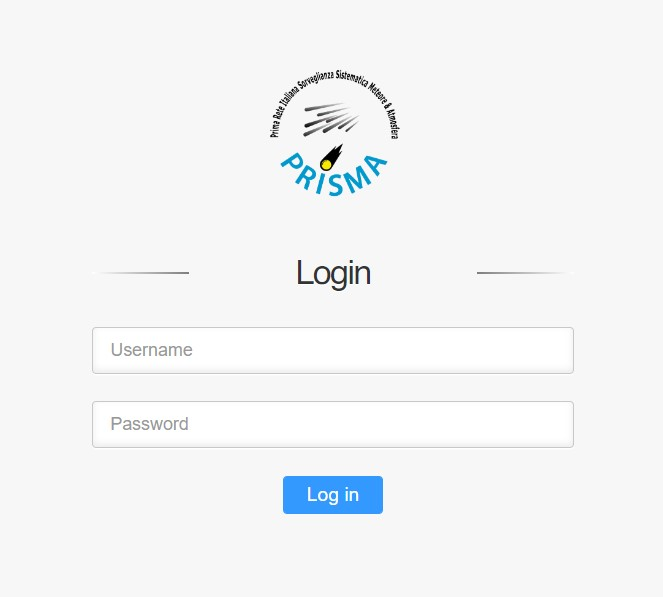
\includegraphics[scale=0.7]{images/login.jpg}
    \caption{Schermata di login.}
    \label{fig:login}
    \end{center}
\end{figure}

Il resto dell'implementazione del sistema è stato oggetto del tirocinio.

\subsection{Menu}

L'utente dopo aver eseguito l'accesso dispone di un menu sulla sinistra per scegliere la sezione di interesse (cfr. figura \ref{fig:menu}). Si noti che alcune funzioni sono nascoste per utenti di livello inferiore (cfr. sezione \ref{sezione-utenti}).

\begin{figure}
    \begin{center}
    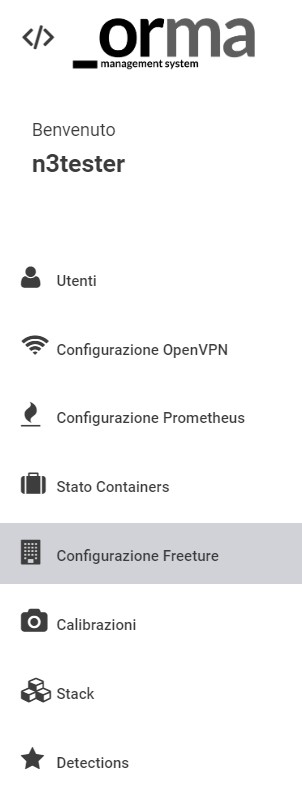
\includegraphics[scale=0.8]{images/menu.jpg}
    \caption{Menu della web application, in questo caso è selezionata la sezione FreeTure.}
    \label{fig:menu}
    \end{center}
\end{figure}